% Options for packages loaded elsewhere
\PassOptionsToPackage{unicode}{hyperref}
\PassOptionsToPackage{hyphens}{url}
%
\documentclass[
]{book}
\usepackage{amsmath,amssymb}
\usepackage{lmodern}
\usepackage{ifxetex,ifluatex}
\ifnum 0\ifxetex 1\fi\ifluatex 1\fi=0 % if pdftex
  \usepackage[T1]{fontenc}
  \usepackage[utf8]{inputenc}
  \usepackage{textcomp} % provide euro and other symbols
\else % if luatex or xetex
  \usepackage{unicode-math}
  \defaultfontfeatures{Scale=MatchLowercase}
  \defaultfontfeatures[\rmfamily]{Ligatures=TeX,Scale=1}
\fi
% Use upquote if available, for straight quotes in verbatim environments
\IfFileExists{upquote.sty}{\usepackage{upquote}}{}
\IfFileExists{microtype.sty}{% use microtype if available
  \usepackage[]{microtype}
  \UseMicrotypeSet[protrusion]{basicmath} % disable protrusion for tt fonts
}{}
\makeatletter
\@ifundefined{KOMAClassName}{% if non-KOMA class
  \IfFileExists{parskip.sty}{%
    \usepackage{parskip}
  }{% else
    \setlength{\parindent}{0pt}
    \setlength{\parskip}{6pt plus 2pt minus 1pt}}
}{% if KOMA class
  \KOMAoptions{parskip=half}}
\makeatother
\usepackage{xcolor}
\IfFileExists{xurl.sty}{\usepackage{xurl}}{} % add URL line breaks if available
\IfFileExists{bookmark.sty}{\usepackage{bookmark}}{\usepackage{hyperref}}
\hypersetup{
  pdftitle={Genome Assembly},
  pdfauthor={officialprofile},
  hidelinks,
  pdfcreator={LaTeX via pandoc}}
\urlstyle{same} % disable monospaced font for URLs
\usepackage{color}
\usepackage{fancyvrb}
\newcommand{\VerbBar}{|}
\newcommand{\VERB}{\Verb[commandchars=\\\{\}]}
\DefineVerbatimEnvironment{Highlighting}{Verbatim}{commandchars=\\\{\}}
% Add ',fontsize=\small' for more characters per line
\usepackage{framed}
\definecolor{shadecolor}{RGB}{248,248,248}
\newenvironment{Shaded}{\begin{snugshade}}{\end{snugshade}}
\newcommand{\AlertTok}[1]{\textcolor[rgb]{0.94,0.16,0.16}{#1}}
\newcommand{\AnnotationTok}[1]{\textcolor[rgb]{0.56,0.35,0.01}{\textbf{\textit{#1}}}}
\newcommand{\AttributeTok}[1]{\textcolor[rgb]{0.77,0.63,0.00}{#1}}
\newcommand{\BaseNTok}[1]{\textcolor[rgb]{0.00,0.00,0.81}{#1}}
\newcommand{\BuiltInTok}[1]{#1}
\newcommand{\CharTok}[1]{\textcolor[rgb]{0.31,0.60,0.02}{#1}}
\newcommand{\CommentTok}[1]{\textcolor[rgb]{0.56,0.35,0.01}{\textit{#1}}}
\newcommand{\CommentVarTok}[1]{\textcolor[rgb]{0.56,0.35,0.01}{\textbf{\textit{#1}}}}
\newcommand{\ConstantTok}[1]{\textcolor[rgb]{0.00,0.00,0.00}{#1}}
\newcommand{\ControlFlowTok}[1]{\textcolor[rgb]{0.13,0.29,0.53}{\textbf{#1}}}
\newcommand{\DataTypeTok}[1]{\textcolor[rgb]{0.13,0.29,0.53}{#1}}
\newcommand{\DecValTok}[1]{\textcolor[rgb]{0.00,0.00,0.81}{#1}}
\newcommand{\DocumentationTok}[1]{\textcolor[rgb]{0.56,0.35,0.01}{\textbf{\textit{#1}}}}
\newcommand{\ErrorTok}[1]{\textcolor[rgb]{0.64,0.00,0.00}{\textbf{#1}}}
\newcommand{\ExtensionTok}[1]{#1}
\newcommand{\FloatTok}[1]{\textcolor[rgb]{0.00,0.00,0.81}{#1}}
\newcommand{\FunctionTok}[1]{\textcolor[rgb]{0.00,0.00,0.00}{#1}}
\newcommand{\ImportTok}[1]{#1}
\newcommand{\InformationTok}[1]{\textcolor[rgb]{0.56,0.35,0.01}{\textbf{\textit{#1}}}}
\newcommand{\KeywordTok}[1]{\textcolor[rgb]{0.13,0.29,0.53}{\textbf{#1}}}
\newcommand{\NormalTok}[1]{#1}
\newcommand{\OperatorTok}[1]{\textcolor[rgb]{0.81,0.36,0.00}{\textbf{#1}}}
\newcommand{\OtherTok}[1]{\textcolor[rgb]{0.56,0.35,0.01}{#1}}
\newcommand{\PreprocessorTok}[1]{\textcolor[rgb]{0.56,0.35,0.01}{\textit{#1}}}
\newcommand{\RegionMarkerTok}[1]{#1}
\newcommand{\SpecialCharTok}[1]{\textcolor[rgb]{0.00,0.00,0.00}{#1}}
\newcommand{\SpecialStringTok}[1]{\textcolor[rgb]{0.31,0.60,0.02}{#1}}
\newcommand{\StringTok}[1]{\textcolor[rgb]{0.31,0.60,0.02}{#1}}
\newcommand{\VariableTok}[1]{\textcolor[rgb]{0.00,0.00,0.00}{#1}}
\newcommand{\VerbatimStringTok}[1]{\textcolor[rgb]{0.31,0.60,0.02}{#1}}
\newcommand{\WarningTok}[1]{\textcolor[rgb]{0.56,0.35,0.01}{\textbf{\textit{#1}}}}
\usepackage{longtable,booktabs,array}
\usepackage{calc} % for calculating minipage widths
% Correct order of tables after \paragraph or \subparagraph
\usepackage{etoolbox}
\makeatletter
\patchcmd\longtable{\par}{\if@noskipsec\mbox{}\fi\par}{}{}
\makeatother
% Allow footnotes in longtable head/foot
\IfFileExists{footnotehyper.sty}{\usepackage{footnotehyper}}{\usepackage{footnote}}
\makesavenoteenv{longtable}
\usepackage{graphicx}
\makeatletter
\def\maxwidth{\ifdim\Gin@nat@width>\linewidth\linewidth\else\Gin@nat@width\fi}
\def\maxheight{\ifdim\Gin@nat@height>\textheight\textheight\else\Gin@nat@height\fi}
\makeatother
% Scale images if necessary, so that they will not overflow the page
% margins by default, and it is still possible to overwrite the defaults
% using explicit options in \includegraphics[width, height, ...]{}
\setkeys{Gin}{width=\maxwidth,height=\maxheight,keepaspectratio}
% Set default figure placement to htbp
\makeatletter
\def\fps@figure{htbp}
\makeatother
\setlength{\emergencystretch}{3em} % prevent overfull lines
\providecommand{\tightlist}{%
  \setlength{\itemsep}{0pt}\setlength{\parskip}{0pt}}
\setcounter{secnumdepth}{5}
\usepackage{booktabs}
\ifluatex
  \usepackage{selnolig}  % disable illegal ligatures
\fi
\usepackage[]{natbib}
\bibliographystyle{apalike}

\title{Genome Assembly}
\author{officialprofile}
\date{2021-09-05}

\begin{document}
\maketitle

{
\setcounter{tocdepth}{1}
\tableofcontents
}
\hypertarget{preface}{%
\chapter{Preface}\label{preface}}

This mini textbook describes selected algorithms that play a main role in the \emph{de novo} genome assembly. The premise of this book is to construct these algorithms from the very bottom and explain step by step the main ideas that stand behind them.

We will try to avoid as mcuch as possible ready-to-use implementations, which are, of course, available, but their use wouldn't serve the educational purpose. Naturally, many applications are included as well.

By default the code is written in R, but at certain points python is also mentioned.

\begin{center}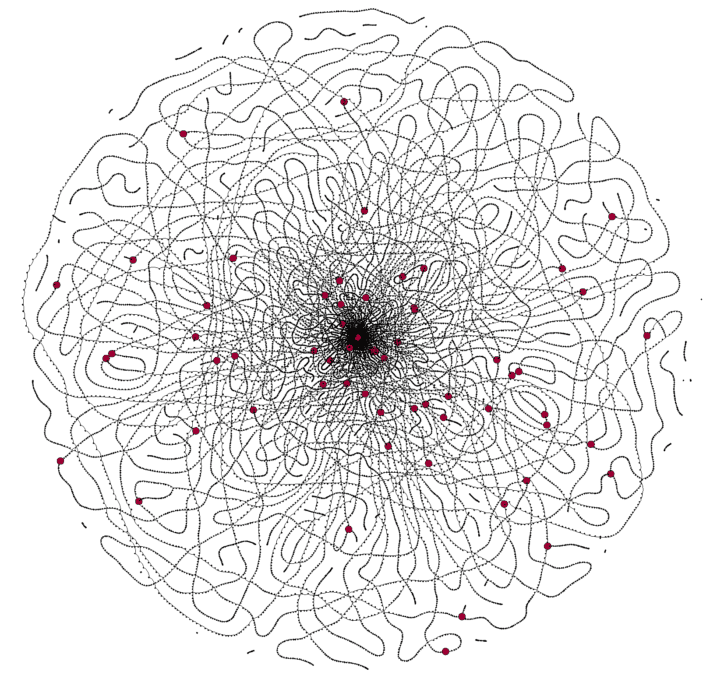
\includegraphics[width=0.8\linewidth]{img/cover} \end{center}

A HiFi De Bruijn graph for a pile of reads from Drosophila genome sequencing. Each dot represents a k-mer (k=23), the edges denote neighboring k-mers. The larger red dots mark the head of heterozygous bubbles. Source: pacb.com.

\hypertarget{prerequisites}{%
\section{Prerequisites}\label{prerequisites}}

It is assumed that the reader

\begin{enumerate}
\def\labelenumi{\arabic{enumi}.}
\item
  has a basic understanding of genetics;
\item
  has some experience with programming in R (is familiar with pipe syntax, etc.)
\item
  had some contact with higher mathematics, e.g.~statistics, graph theory.
\end{enumerate}

Throughout the book the following libraries are being used and it is assumed that the reader has them loaded.

\begin{Shaded}
\begin{Highlighting}[]
\FunctionTok{library}\NormalTok{(stringr)}
\FunctionTok{library}\NormalTok{(dplyr)}
\FunctionTok{library}\NormalTok{(igraph)}
\end{Highlighting}
\end{Shaded}

\hypertarget{introduction}{%
\chapter{Introduction to genome assembly}\label{introduction}}

Genome assembly has been regarded as one of the most important and most challenging problems in bioinformatics, at least since the late 80's, when the Human Genome Project was announced.

Genomes tend to be almost inconceivably long. Human DNA for example is approximately thousand times longer than the Bible, and some species have their genome even dozens times longer than ours. Yet the algorithmic part of the problem arises not mainly because of their length. This was definitely the case for the biotechnologicians, who few decades ago were constrained within insufficiently effective sequencing techniques. From bioinformaticians perspective though the core of the problem is located deeper.

A good analogy, explaining the nature of the challenge, is a schredded newspaper. De novo assembly resembles reconstruction of the original document from a set of its unarranged pieces, like on the figure below.

As one can imagine the problem is difficult, but not because the newspaper has twenty or fourty pages. If we had just one the assembly still wouldn't be easy. The length of the genome, although far from being irrelevant, is for us more of a secondary issue. On the other hand, repetitive patterns, which for biotechnologicians are not a problem at all, will complicate our journey substantially. Reader will perhaps come up to the very similar conclusions as the succeeding topics will uncover.

One should also underline the fact that transcriptome assembly is not the same as the genome assembly. Read coverage of the latter is relatively uniform, whereas transcriptome can be differentially expressed and therefore the frequency of its reads can vary a lot. In genome assembly non-uniform abundance of the reads simply indicates existence of repetitions. In the case of transcription product it is much less straightforward. Methods that overcome this issue exist but they are beyond of the scope of this textbook.

\hypertarget{basic}{%
\chapter{Basic string manipulations}\label{basic}}

Before we dive into the main topics let's warm up with few basic exercises. On the one hand some of these problems might be regarded as a form of general familiarization with string manipulations. Being able to get through them is in a sense a must, at least from a perspective of algorithms that will be discussed later. On the other hand some of the problems, like generating k-mers or suffixes, are absolutely crucial in genome assembly and one has to know them to a tee. So, without further ado, let's do the warm up.

\hypertarget{generating-random-dna-sequence}{%
\section{Generating random DNA sequence}\label{generating-random-dna-sequence}}

Let's start with writing a function that, for a given integer n \textgreater{} 0, returns randomly generated DNA sequence.

\begin{Shaded}
\begin{Highlighting}[]
\NormalTok{random\_sequence }\OtherTok{\textless{}{-}} \ControlFlowTok{function}\NormalTok{(n)\{}
  \FunctionTok{return}\NormalTok{(}\FunctionTok{sample}\NormalTok{(}\FunctionTok{c}\NormalTok{(}\StringTok{\textquotesingle{}A\textquotesingle{}}\NormalTok{,}\StringTok{\textquotesingle{}C\textquotesingle{}}\NormalTok{,}\StringTok{\textquotesingle{}G\textquotesingle{}}\NormalTok{,}\StringTok{\textquotesingle{}T\textquotesingle{}}\NormalTok{), n, }\AttributeTok{replace =} \ConstantTok{TRUE}\NormalTok{))}
\NormalTok{\}}

\FunctionTok{random\_sequence}\NormalTok{(}\DecValTok{10}\NormalTok{)}
\CommentTok{\#\textgreater{}  [1] "G" "A" "C" "C" "G" "T" "G" "A" "T" "C"}
\end{Highlighting}
\end{Shaded}

If we want our returned sequence to be in a form of a single string we can use \texttt{paste()} function with collapse parameter equal to \texttt{\textquotesingle{}\textquotesingle{}}.

\begin{Shaded}
\begin{Highlighting}[]
\FunctionTok{paste}\NormalTok{(}\FunctionTok{random\_sequence}\NormalTok{(}\DecValTok{10}\NormalTok{), }\AttributeTok{collapse =} \StringTok{\textquotesingle{}\textquotesingle{}}\NormalTok{)}
\CommentTok{\#\textgreater{} [1] "TCAACACTCG"}
\end{Highlighting}
\end{Shaded}

For now we will try to stick to the first form, mainly because base R is not that good at manipulating strings (at this point we try to not employ any additional libraries like stringr). If a \texttt{DNA} is equal to \texttt{\textquotesingle{}ACGTG\textquotesingle{}} then we won't get a substring \texttt{\textquotesingle{}CG\textquotesingle{}} simply by writing \texttt{DNA{[}2:3{]}} (one could to this in python). On the other hand, if DNA is a vector \texttt{c(\textquotesingle{}A\textquotesingle{},\ \textquotesingle{}C\textquotesingle{},\ \textquotesingle{}G\textquotesingle{},\ \textquotesingle{}T\textquotesingle{},\ \textquotesingle{}G\textquotesingle{})} then \texttt{DNA{[}2:3{]}} will return \texttt{c(\textquotesingle{}C\textquotesingle{},\ \textquotesingle{}G\textquotesingle{})} that in turn can be easily merged into \texttt{\textquotesingle{}CG\textquotesingle{}}.

\hypertarget{finding-cdna}{%
\section{Finding cDNA}\label{finding-cdna}}

One must know that C (cytosine) is complementary to G (guanine), and A (adenine) is complementary to T (thymine). In order to create a cDNA we will at first construct a list (in Python it would be a dictionary) of complementary nucleobases.

\begin{Shaded}
\begin{Highlighting}[]
\NormalTok{c\_bases }\OtherTok{\textless{}{-}} \FunctionTok{list}\NormalTok{(}\StringTok{\textquotesingle{}A\textquotesingle{}} \OtherTok{=} \StringTok{\textquotesingle{}T\textquotesingle{}}\NormalTok{, }\StringTok{\textquotesingle{}C\textquotesingle{}} \OtherTok{=} \StringTok{\textquotesingle{}G\textquotesingle{}}\NormalTok{, }\StringTok{\textquotesingle{}G\textquotesingle{}} \OtherTok{=} \StringTok{\textquotesingle{}C\textquotesingle{}}\NormalTok{, }\StringTok{\textquotesingle{}T\textquotesingle{}} \OtherTok{=} \StringTok{\textquotesingle{}A\textquotesingle{}}\NormalTok{)}

\NormalTok{c\_bases[}\StringTok{\textquotesingle{}A\textquotesingle{}}\NormalTok{][[}\DecValTok{1}\NormalTok{]]}
\CommentTok{\#\textgreater{} [1] "T"}
\end{Highlighting}
\end{Shaded}

This data structure will allows us to directly pull out complementary bases. Let's build a function utilizes this.

\begin{Shaded}
\begin{Highlighting}[]
\NormalTok{complementary\_sequence }\OtherTok{\textless{}{-}} \ControlFlowTok{function}\NormalTok{(sequence)\{}
\NormalTok{  complementary }\OtherTok{=} \FunctionTok{c}\NormalTok{()}
  \ControlFlowTok{for}\NormalTok{ (base }\ControlFlowTok{in}\NormalTok{ sequence)\{}
\NormalTok{    complementary }\OtherTok{=} \FunctionTok{c}\NormalTok{(complementary, c\_bases[base][[}\DecValTok{1}\NormalTok{]])}
\NormalTok{  \}}
  \FunctionTok{return}\NormalTok{(complementary)}
\NormalTok{\}}
\end{Highlighting}
\end{Shaded}

Please note that we append complementary nucleobase in a seemingly non-optimal way, namely \texttt{sequence\ =\ c(sequence,\ new\_nucleobase)}. One could argue that this should be done with \texttt{append()}, i. e. \texttt{sequence\ =\ append(sequence,\ new\_nucleobase)}, but in fact the append in R is regarded as a relatively slow function and our solution is usually more recommended.

\begin{Shaded}
\begin{Highlighting}[]
\NormalTok{seq }\OtherTok{\textless{}{-}} \FunctionTok{random\_sequence}\NormalTok{(}\DecValTok{20}\NormalTok{)}
\FunctionTok{cat}\NormalTok{(}\StringTok{\textquotesingle{} DNA =\textquotesingle{}}\NormalTok{, seq, }\StringTok{\textquotesingle{}}\SpecialCharTok{\textbackslash{}n}\StringTok{\textquotesingle{}}\NormalTok{)}
\CommentTok{\#\textgreater{}  DNA = G T C G C G C T C T A G A G G T C G G G}
\NormalTok{cseq }\OtherTok{\textless{}{-}} \FunctionTok{complementary\_sequence}\NormalTok{(seq)}
\FunctionTok{cat}\NormalTok{(}\StringTok{\textquotesingle{}cDNA =\textquotesingle{}}\NormalTok{, cseq)}
\CommentTok{\#\textgreater{} cDNA = C A G C G C G A G A T C T C C A G C C C}
\end{Highlighting}
\end{Shaded}

There is also a neater way to compute, and in a way avoid, these kind of loops. One can achieve this though functions like \texttt{apply()}, \texttt{sapply()} or \texttt{lapply()}.

\begin{Shaded}
\begin{Highlighting}[]
\NormalTok{complementary\_sequence }\OtherTok{\textless{}{-}} \ControlFlowTok{function}\NormalTok{(sequence)\{}
  \FunctionTok{sapply}\NormalTok{(seq, }\ControlFlowTok{function}\NormalTok{(base) c\_bases[base][[}\DecValTok{1}\NormalTok{]])}
\NormalTok{\}}
\end{Highlighting}
\end{Shaded}

The clear downside of using functions like the one above is loss of legibility. Applying them can also be not as straightforward and intuitive as writing a conventional loop. Advanced programmers though find these functions very handy, fast and as readable as standard for or while loop. For that reason we will try to balance these two approaches out. We don't want our code to be too hermetic, but also we should not limit ourselves by deliberately avoiding legitimate solutions.

\hypertarget{finding-reverse-complementary}{%
\section{Finding reverse complementary}\label{finding-reverse-complementary}}

Obtaining reverse complementary is very similar. The only difference is that instead of appending complementary nucleobases we will prepend them.

\begin{Shaded}
\begin{Highlighting}[]
\NormalTok{reverse\_complementary }\OtherTok{\textless{}{-}} \ControlFlowTok{function}\NormalTok{(sequence)\{}
\NormalTok{  reverse }\OtherTok{=} \FunctionTok{c}\NormalTok{()}
  \ControlFlowTok{for}\NormalTok{ (base }\ControlFlowTok{in}\NormalTok{ sequence)\{}
\NormalTok{    reverse }\OtherTok{=} \FunctionTok{c}\NormalTok{(c\_bases[base][[}\DecValTok{1}\NormalTok{]], reverse)}
\NormalTok{  \}}
  \FunctionTok{return}\NormalTok{(reverse)}
\NormalTok{\}}
\end{Highlighting}
\end{Shaded}

\begin{Shaded}
\begin{Highlighting}[]
\NormalTok{seq }\OtherTok{\textless{}{-}} \FunctionTok{random\_sequence}\NormalTok{(}\DecValTok{20}\NormalTok{)}
\FunctionTok{cat}\NormalTok{(}\StringTok{\textquotesingle{} DNA =\textquotesingle{}}\NormalTok{, seq, }\StringTok{\textquotesingle{}}\SpecialCharTok{\textbackslash{}n}\StringTok{\textquotesingle{}}\NormalTok{)}
\CommentTok{\#\textgreater{}  DNA = A G T C C A G C C G T G C A C T A C T T}
\NormalTok{rcseq }\OtherTok{\textless{}{-}} \FunctionTok{reverse\_complementary}\NormalTok{(seq)}
\FunctionTok{cat}\NormalTok{(}\StringTok{\textquotesingle{}cDNA =\textquotesingle{}}\NormalTok{, rcseq)}
\CommentTok{\#\textgreater{} cDNA = A A G T A G T G C A C G G C T G G A C T}
\end{Highlighting}
\end{Shaded}

\hypertarget{graph}{%
\chapter{Graph theory}\label{graph}}

\hypertarget{bruijn}{%
\chapter{De Bruijn graph}\label{bruijn}}

\hypertarget{bwt}{%
\chapter{Burrows-Wheeler transform}\label{bwt}}

The Burrows-Wheeler transform is one of the most effective lossless text compression method available. It provides a reversible transformation for text that makes it easier to compress. Of course, one may wonder what text compression has to do with genome assembly. As a matter of fact these two issues are closely related. But we should to be more precise here - text compression is closely related to pattern matching which in turn is crucial for the genome assembly. In a broad sense compression algorithms look for patterns and try to remove repetitions. We want to take advantage of this feature, especially because repetitive patterns tend to be very abundant in genomic sequences.

It is worth mentioning that the Burrows-Wheeler transform is also closely related to suffix trees and suffix arrays, which are commonly used within pattern matching. This relationship will be studied later but perhaps reader should already keep the trivia in mind. \citep{bw1}

\hypertarget{introduction-1}{%
\section{Introduction}\label{introduction-1}}

The Burrows-Wheeler transform method is often referred to as ``block sorting'', because it takes a block of text and permutes it. By permuting a block of text we mean rearranging the order of its symbols. Once again, we should be more precise here because Burrows-Wheeler transform performes a specific type of permutation, namely \emph{circural shift permutation}: all of the characters are moved one position to the left, and first character moves to the last position.

\hypertarget{burrows-wheeler-matrix}{%
\section{Burrows-Wheeler matrix}\label{burrows-wheeler-matrix}}

Consider the following sequence:

\begin{Shaded}
\begin{Highlighting}[numbers=left,,]
\NormalTok{sequence }\OtherTok{\textless{}{-}} \StringTok{\textquotesingle{}GATTACA\textquotesingle{}}
\end{Highlighting}
\end{Shaded}

In order to create the Burrows-Wheeler matrix, from which the transform itself can be obtained, for the given string we at first add the dollar sign \$ at the end of the sequence.

\begin{Shaded}
\begin{Highlighting}[numbers=left,,]
\NormalTok{sequence  }\OtherTok{\textless{}{-}} \FunctionTok{str\_c}\NormalTok{(sequence, }\StringTok{\textquotesingle{}$\textquotesingle{}}\NormalTok{)}
\end{Highlighting}
\end{Shaded}

Afterwards we perform a series of circular shift permutations.

\begin{Shaded}
\begin{Highlighting}[numbers=left,,]
\NormalTok{sequences }\OtherTok{\textless{}{-}} \FunctionTok{c}\NormalTok{(sequence)}
\NormalTok{n         }\OtherTok{\textless{}{-}} \FunctionTok{nchar}\NormalTok{(sequence)}

\ControlFlowTok{for}\NormalTok{ (i }\ControlFlowTok{in} \DecValTok{1}\SpecialCharTok{:}\NormalTok{(n}\DecValTok{{-}1}\NormalTok{))\{}
\NormalTok{  sequence }\OtherTok{\textless{}{-}} \FunctionTok{str\_c}\NormalTok{(}\FunctionTok{str\_sub}\NormalTok{(sequence, }\DecValTok{2}\NormalTok{, n),}
                    \FunctionTok{str\_sub}\NormalTok{(sequence, }\DecValTok{1}\NormalTok{, }\DecValTok{1}\NormalTok{))}
  
\NormalTok{  sequences }\OtherTok{\textless{}{-}} \FunctionTok{c}\NormalTok{(sequences, sequence)}
\NormalTok{\}}

\FunctionTok{cat}\NormalTok{(sequences, }\AttributeTok{sep =} \StringTok{\textquotesingle{}}\SpecialCharTok{\textbackslash{}n}\StringTok{\textquotesingle{}}\NormalTok{)}
\CommentTok{\#\textgreater{} GATTACA$}
\CommentTok{\#\textgreater{} ATTACA$G}
\CommentTok{\#\textgreater{} TTACA$GA}
\CommentTok{\#\textgreater{} TACA$GAT}
\CommentTok{\#\textgreater{} ACA$GATT}
\CommentTok{\#\textgreater{} CA$GATTA}
\CommentTok{\#\textgreater{} A$GATTAC}
\CommentTok{\#\textgreater{} $GATTACA}
\end{Highlighting}
\end{Shaded}

Then we sort these sequences with the assumption that the dollar sign precedes lexicographically every other symbol.

\begin{Shaded}
\begin{Highlighting}[numbers=left,,]
\NormalTok{sequences }\OtherTok{\textless{}{-}} \FunctionTok{sort}\NormalTok{(sequences) }
\FunctionTok{cat}\NormalTok{(sequences, }\AttributeTok{sep =} \StringTok{\textquotesingle{}}\SpecialCharTok{\textbackslash{}n}\StringTok{\textquotesingle{}}\NormalTok{)}
\CommentTok{\#\textgreater{} $GATTACA}
\CommentTok{\#\textgreater{} A$GATTAC}
\CommentTok{\#\textgreater{} ACA$GATT}
\CommentTok{\#\textgreater{} ATTACA$G}
\CommentTok{\#\textgreater{} CA$GATTA}
\CommentTok{\#\textgreater{} GATTACA$}
\CommentTok{\#\textgreater{} TACA$GAT}
\CommentTok{\#\textgreater{} TTACA$GA}
\end{Highlighting}
\end{Shaded}

For our convenience let's split these permutations into vectors of single characters.

\begin{Shaded}
\begin{Highlighting}[numbers=left,,]
\NormalTok{bw.matrix           }\OtherTok{\textless{}{-}} \FunctionTok{data.frame}\NormalTok{(}\FunctionTok{matrix}\NormalTok{(, n, n))}
\FunctionTok{colnames}\NormalTok{(bw.matrix) }\OtherTok{\textless{}{-}} \DecValTok{1}\SpecialCharTok{:}\NormalTok{n}

\ControlFlowTok{for}\NormalTok{ (i }\ControlFlowTok{in} \DecValTok{1}\SpecialCharTok{:}\NormalTok{n)\{}
\NormalTok{  bw.matrix[i, ] }\OtherTok{\textless{}{-}} \FunctionTok{strsplit}\NormalTok{(sequences[i], }\AttributeTok{split =} \StringTok{\textquotesingle{}\textquotesingle{}}\NormalTok{)[[}\DecValTok{1}\NormalTok{]]}
\NormalTok{\}}

\NormalTok{knitr}\SpecialCharTok{::}\FunctionTok{kable}\NormalTok{(bw.matrix)}
\end{Highlighting}
\end{Shaded}

\begin{tabular}{l|l|l|l|l|l|l|l}
\hline
1 & 2 & 3 & 4 & 5 & 6 & 7 & 8\\
\hline
\$ & G & A & T & T & A & C & A\\
\hline
A & \$ & G & A & T & T & A & C\\
\hline
A & C & A & \$ & G & A & T & T\\
\hline
A & T & T & A & C & A & \$ & G\\
\hline
C & A & \$ & G & A & T & T & A\\
\hline
G & A & T & T & A & C & A & \$\\
\hline
T & A & C & A & \$ & G & A & T\\
\hline
T & T & A & C & A & \$ & G & A\\
\hline
\end{tabular}

Thus we have created the \textbf{Burrows-Wheeler matrix}. Sequence in the last column is called the \textbf{Burrows-Wheeler transform}.

\begin{Shaded}
\begin{Highlighting}[numbers=left,,]
\NormalTok{transform }\OtherTok{\textless{}{-}} \FunctionTok{paste}\NormalTok{(bw.matrix[,n], }\AttributeTok{collapse =} \StringTok{\textquotesingle{}\textquotesingle{}}\NormalTok{)}

\FunctionTok{cat}\NormalTok{(}\StringTok{\textquotesingle{}The Burrows{-}Wheeler transform of\textquotesingle{}}\NormalTok{, }
\NormalTok{    sequence, }\StringTok{\textquotesingle{}is\textquotesingle{}}\NormalTok{, transform)}
\CommentTok{\#\textgreater{} The Burrows{-}Wheeler transform of $GATTACA is ACTGA$TA}
\end{Highlighting}
\end{Shaded}

\hypertarget{inverse-transform}{%
\section{Inverse transform}\label{inverse-transform}}

As we said at the very beginning the transform is reversible. Having only the transformed sequence we are going to reconstruct the Burrows-Wheeler matrix and initial sequence itself.

Firstly let's sort the characters of the transformed sequence.

\begin{Shaded}
\begin{Highlighting}[numbers=left,,]
\NormalTok{first.sequence }\OtherTok{\textless{}{-}} \FunctionTok{strsplit}\NormalTok{(transform, }\AttributeTok{split =} \StringTok{\textquotesingle{}\textquotesingle{}}\NormalTok{)[[}\DecValTok{1}\NormalTok{]] }\SpecialCharTok{\%\textgreater{}\%}\NormalTok{ sort}
\FunctionTok{paste}\NormalTok{(first.sequence, }\AttributeTok{collapse =} \StringTok{\textquotesingle{}\textquotesingle{}}\NormalTok{)}
\CommentTok{\#\textgreater{} [1] "$AAACGTT"}
\end{Highlighting}
\end{Shaded}

Note that this string is equivalent to the first column of the Burrrows-Wheeler transform.

\begin{Shaded}
\begin{Highlighting}[numbers=left,,]
\NormalTok{bw.inverse           }\OtherTok{\textless{}{-}} \FunctionTok{data.frame}\NormalTok{(}\FunctionTok{matrix}\NormalTok{(, n, }\DecValTok{2}\NormalTok{))}
\FunctionTok{colnames}\NormalTok{(bw.inverse) }\OtherTok{\textless{}{-}} \FunctionTok{c}\NormalTok{(n, }\DecValTok{1}\NormalTok{)}

\NormalTok{bw.inverse[, }\DecValTok{1}\NormalTok{] }\OtherTok{\textless{}{-}} \FunctionTok{strsplit}\NormalTok{(transform, }\AttributeTok{split =} \StringTok{\textquotesingle{}\textquotesingle{}}\NormalTok{)[[}\DecValTok{1}\NormalTok{]]}
\NormalTok{bw.inverse[ ,}\DecValTok{2}\NormalTok{] }\OtherTok{\textless{}{-}}\NormalTok{ first.sequence}

\NormalTok{knitr}\SpecialCharTok{::}\FunctionTok{kable}\NormalTok{(bw.inverse)}
\end{Highlighting}
\end{Shaded}

\begin{tabular}{l|l}
\hline
8 & 1\\
\hline
A & \$\\
\hline
C & A\\
\hline
T & A\\
\hline
G & A\\
\hline
A & C\\
\hline
\$ & G\\
\hline
T & T\\
\hline
A & T\\
\hline
\end{tabular}

Also keep in mind that the characters from last and the first column are adjacent. In other words, at this point we have a set of 2-mers.

\begin{Shaded}
\begin{Highlighting}[numbers=left,,]
\NormalTok{kmers }\OtherTok{\textless{}{-}} \FunctionTok{apply}\NormalTok{(bw.inverse, }\DecValTok{1}\NormalTok{, }
               \ControlFlowTok{function}\NormalTok{(x) }\FunctionTok{paste}\NormalTok{(x, }\AttributeTok{collapse =} \StringTok{\textquotesingle{}\textquotesingle{}}\NormalTok{))}
\NormalTok{kmers}
\CommentTok{\#\textgreater{} [1] "A$" "CA" "TA" "GA" "AC" "$G" "TT" "AT"}
\end{Highlighting}
\end{Shaded}

The reconstruction process strictly relies on the fact that Burrows-Wheeler matrix is sorted lexicographically. This property will allow us to retrieve the remaining columns.

\begin{Shaded}
\begin{Highlighting}[numbers=left,,]
\NormalTok{kmers }\OtherTok{\textless{}{-}} \FunctionTok{sort}\NormalTok{(kmers)}
\NormalTok{kmers}
\CommentTok{\#\textgreater{} [1] "$G" "A$" "AC" "AT" "CA" "GA" "TA" "TT"}
\end{Highlighting}
\end{Shaded}

The 2-mers (k-mers in general) that we sorted lexicographically represent first two columns of the Burrows-Wheeler matrix. We can extract last character of each 2-mer in the following way:

\begin{Shaded}
\begin{Highlighting}[numbers=left,,]
\FunctionTok{sapply}\NormalTok{(kmers, }\ControlFlowTok{function}\NormalTok{(x) }\FunctionTok{str\_sub}\NormalTok{(x, }\DecValTok{2}\NormalTok{, }\DecValTok{2}\NormalTok{), }
       \AttributeTok{simplify =} \ConstantTok{TRUE}\NormalTok{, }\AttributeTok{USE.NAMES =} \ConstantTok{FALSE}\NormalTok{)}
\CommentTok{\#\textgreater{} [1] "G" "$" "C" "T" "A" "A" "A" "T"}
\end{Highlighting}
\end{Shaded}

By inserting this set of characters we obtained the second column, and by iterating the proccess of building substrings, sorting them, and retrieving last characters we can fill the whole Burrows-Wheeler matrix.

\begin{Shaded}
\begin{Highlighting}[numbers=left,,]
\ControlFlowTok{for}\NormalTok{ (i }\ControlFlowTok{in} \DecValTok{2}\SpecialCharTok{:}\NormalTok{(n}\DecValTok{{-}1}\NormalTok{))\{}
\NormalTok{  kmers             }\OtherTok{\textless{}{-}} \FunctionTok{apply}\NormalTok{(bw.inverse, }\DecValTok{1}\NormalTok{, }
                             \ControlFlowTok{function}\NormalTok{(x) }\FunctionTok{paste}\NormalTok{(x, }\AttributeTok{collapse =} \StringTok{\textquotesingle{}\textquotesingle{}}\NormalTok{))}
\NormalTok{  kmers             }\OtherTok{\textless{}{-}} \FunctionTok{sort}\NormalTok{(kmers)}
\NormalTok{  bw.inverse[, i}\SpecialCharTok{+}\DecValTok{1}\NormalTok{] }\OtherTok{\textless{}{-}} \FunctionTok{sapply}\NormalTok{(kmers, }\ControlFlowTok{function}\NormalTok{(x) }\FunctionTok{str\_sub}\NormalTok{(x, i, i), }
                              \AttributeTok{simplify =} \ConstantTok{TRUE}\NormalTok{, }\AttributeTok{USE.NAMES =} \ConstantTok{FALSE}\NormalTok{)}
  \FunctionTok{colnames}\NormalTok{(bw.inverse)[i}\SpecialCharTok{+}\DecValTok{1}\NormalTok{] }\OtherTok{=}\NormalTok{ i}
\NormalTok{\}}
\NormalTok{knitr}\SpecialCharTok{::}\FunctionTok{kable}\NormalTok{(bw.inverse)}
\end{Highlighting}
\end{Shaded}

\begin{tabular}{l|l|l|l|l|l|l|l}
\hline
8 & 1 & 2 & 3 & 4 & 5 & 6 & 7\\
\hline
A & \$ & G & A & T & T & A & C\\
\hline
C & A & \$ & G & A & T & T & A\\
\hline
T & A & C & A & \$ & G & A & T\\
\hline
G & A & T & T & A & C & A & \$\\
\hline
A & C & A & \$ & G & A & T & T\\
\hline
\$ & G & A & T & T & A & C & A\\
\hline
T & T & A & C & A & \$ & G & A\\
\hline
A & T & T & A & C & A & \$ & G\\
\hline
\end{tabular}

Finally we move first column to the very end

\begin{Shaded}
\begin{Highlighting}[numbers=left,,]
\NormalTok{bw.inverse[,n}\SpecialCharTok{+}\DecValTok{1}\NormalTok{] }\OtherTok{\textless{}{-}}\NormalTok{ bw.inverse[, }\DecValTok{1}\NormalTok{]}
\NormalTok{bw.inverse       }\OtherTok{\textless{}{-}}\NormalTok{ bw.inverse[,}\DecValTok{2}\SpecialCharTok{:}\NormalTok{(n}\SpecialCharTok{+}\DecValTok{1}\NormalTok{)]}
\FunctionTok{colnames}\NormalTok{(bw.inverse)[n] }\OtherTok{=}\NormalTok{ n}

\NormalTok{knitr}\SpecialCharTok{::}\FunctionTok{kable}\NormalTok{(bw.inverse)}
\end{Highlighting}
\end{Shaded}

\begin{tabular}{l|l|l|l|l|l|l|l}
\hline
1 & 2 & 3 & 4 & 5 & 6 & 7 & 8\\
\hline
\$ & G & A & T & T & A & C & A\\
\hline
A & \$ & G & A & T & T & A & C\\
\hline
A & C & A & \$ & G & A & T & T\\
\hline
A & T & T & A & C & A & \$ & G\\
\hline
C & A & \$ & G & A & T & T & A\\
\hline
G & A & T & T & A & C & A & \$\\
\hline
T & A & C & A & \$ & G & A & T\\
\hline
T & T & A & C & A & \$ & G & A\\
\hline
\end{tabular}

One can also verify that bw.matrix and bw.inverse are in fact the same.

\begin{Shaded}
\begin{Highlighting}[numbers=left,,]
\NormalTok{knitr}\SpecialCharTok{::}\FunctionTok{kable}\NormalTok{(bw.inverse }\SpecialCharTok{==}\NormalTok{ bw.matrix)}
\end{Highlighting}
\end{Shaded}

\begin{tabular}{l|l|l|l|l|l|l|l}
\hline
1 & 2 & 3 & 4 & 5 & 6 & 7 & 8\\
\hline
TRUE & TRUE & TRUE & TRUE & TRUE & TRUE & TRUE & TRUE\\
\hline
TRUE & TRUE & TRUE & TRUE & TRUE & TRUE & TRUE & TRUE\\
\hline
TRUE & TRUE & TRUE & TRUE & TRUE & TRUE & TRUE & TRUE\\
\hline
TRUE & TRUE & TRUE & TRUE & TRUE & TRUE & TRUE & TRUE\\
\hline
TRUE & TRUE & TRUE & TRUE & TRUE & TRUE & TRUE & TRUE\\
\hline
TRUE & TRUE & TRUE & TRUE & TRUE & TRUE & TRUE & TRUE\\
\hline
TRUE & TRUE & TRUE & TRUE & TRUE & TRUE & TRUE & TRUE\\
\hline
TRUE & TRUE & TRUE & TRUE & TRUE & TRUE & TRUE & TRUE\\
\hline
\end{tabular}

Additionally we can encapsulate the Burrows-Wheeler transform in a form of a single function.

\begin{Shaded}
\begin{Highlighting}[numbers=left,,]
\NormalTok{BWT }\OtherTok{\textless{}{-}} \ControlFlowTok{function}\NormalTok{(sequence)\{}
\NormalTok{  sequence  }\OtherTok{\textless{}{-}} \FunctionTok{str\_c}\NormalTok{(sequence, }\StringTok{\textquotesingle{}$\textquotesingle{}}\NormalTok{)}
\NormalTok{  sequences }\OtherTok{\textless{}{-}} \FunctionTok{c}\NormalTok{(sequence)}
\NormalTok{  n         }\OtherTok{\textless{}{-}} \FunctionTok{nchar}\NormalTok{(sequence)}

  \ControlFlowTok{for}\NormalTok{ (i }\ControlFlowTok{in} \DecValTok{1}\SpecialCharTok{:}\NormalTok{(n}\DecValTok{{-}1}\NormalTok{))\{}
\NormalTok{    sequence }\OtherTok{\textless{}{-}} \FunctionTok{str\_c}\NormalTok{(}\FunctionTok{str\_sub}\NormalTok{(sequence, }\DecValTok{2}\NormalTok{, n),}
                     \FunctionTok{str\_sub}\NormalTok{(sequence, }\DecValTok{1}\NormalTok{, }\DecValTok{1}\NormalTok{))}
\NormalTok{    sequences }\OtherTok{\textless{}{-}} \FunctionTok{c}\NormalTok{(sequences, sequence)}
\NormalTok{  \}}
\NormalTok{  sequences }\OtherTok{\textless{}{-}} \FunctionTok{sort}\NormalTok{(sequences) }
  
\NormalTok{  bw.matrix           }\OtherTok{\textless{}{-}} \FunctionTok{data.frame}\NormalTok{(}\FunctionTok{matrix}\NormalTok{(, n, n))}
  \FunctionTok{colnames}\NormalTok{(bw.matrix) }\OtherTok{\textless{}{-}} \DecValTok{1}\SpecialCharTok{:}\NormalTok{n}

  \ControlFlowTok{for}\NormalTok{ (i }\ControlFlowTok{in} \DecValTok{1}\SpecialCharTok{:}\NormalTok{n)\{}
\NormalTok{    bw.matrix[i, ] }\OtherTok{\textless{}{-}} \FunctionTok{strsplit}\NormalTok{(sequences[i], }\AttributeTok{split =} \StringTok{\textquotesingle{}\textquotesingle{}}\NormalTok{)[[}\DecValTok{1}\NormalTok{]]}
\NormalTok{  \}}
  \FunctionTok{return}\NormalTok{(}\FunctionTok{paste}\NormalTok{(bw.matrix[,n], }\AttributeTok{collapse =} \StringTok{\textquotesingle{}\textquotesingle{}}\NormalTok{))}
\NormalTok{\}}
\end{Highlighting}
\end{Shaded}

\begin{Shaded}
\begin{Highlighting}[numbers=left,,]
\FunctionTok{BWT}\NormalTok{(}\StringTok{\textquotesingle{}GATTACA\textquotesingle{}}\NormalTok{)}
\CommentTok{\#\textgreater{} [1] "ACTGA$TA"}
\end{Highlighting}
\end{Shaded}

One can verify that this output is equal to result we obtained earlier.

Out of pure curiosity lets check the Burrows-Wheeler transform for a longer sequence.

\begin{Shaded}
\begin{Highlighting}[numbers=left,,]
\FunctionTok{BWT}\NormalTok{(}\StringTok{\textquotesingle{}ATGCTCGTGCCATCATATAGCGCGCGCGCGATCTCTACGCGCG\textquotesingle{}}\NormalTok{)}
\CommentTok{\#\textgreater{} [1] "GTTTCCG$TCGGGGGAGGGTTGTCCTCCCCCCATCCAAACCAGA"}
\end{Highlighting}
\end{Shaded}

Please note that the input string has no identical characters at adjacent positions, whereas in the transformed sequence such situation appears quite often. These substrings of identical characters will allow us represent the sequence in a more condensed manner and expediate pattern matching.

  \bibliography{book.bib,packages.bib}

\end{document}
